\documentclass[12pt,a4paper,titlepage]{article}
\usepackage[italian]{babel}
\usepackage[T1]{fontenc}
\usepackage[latin1]{inputenc}
\usepackage{titlesec}
\usepackage[hidelinks]{hyperref}
\usepackage[a4paper,top=2cm,bottom=2cm,left=1cm,right=1cm]{geometry}
\usepackage{soulutf8,color}
\usepackage{emptypage}                     
\usepackage{fancyhdr}
\usepackage{graphicx}
\usepackage{float}
\pagestyle{fancy}

\begin{document}

\title{ANALISI DEI REQUISITI}
\author{SWEg Group}
\date{}
\maketitle

\lhead{SWEg Group}
\chead{}
\lfoot{Analisi dei Requisiti}
\cfoot{}
\rfoot{\thepage}
\renewcommand{\headrulewidth}{0.2pt}
\renewcommand{\footrulewidth}{0.2pt}
\rhead{Registro Modifiche}
\section{Registro Modifiche}
\small %rippicciolisce il testo

{\renewcommand\arraystretch{1.2}  %aumenta l'altezza di ogni riga
\begin{tabular}{|l|c|c|c|}
	\hline
	{\textbf{Modifica}}&{\textbf{Nome}}&{\textbf{Data}}&{\textbf{Ver.}}\\
	\hline
	Creazione Raw Documento & Gianluca Crivellaro & 21/12/2016 & 0.0.1 \\
	\hline
	Modifica Raw & Gianluca Crivellaro & 22/12/2016 & 0.0.2 \\
	\hline
	Aggiunti Requisiti & Sebastiano Marchesini & 23/12/2016 & 0.0.3 \\
	\hline
	Aggiunti Requisiti Estesi Concordati & Gianluca Crivellaro & 27/12/2016 & 0.0.4 \\
	\hline
	Stesura Documento (Introduzione) & Sebastiano Marchesini &  28/12/2016 & 0.1.0 \\
	\hline
	Creazione Grafici UML & Pietro Lonardi e Gianluca C. & 29/12/2016 & 0.1.1 \\
	\hline
	Stesura Documento (Descrizione Generale \& Casi d'Uso) & Sebastiano Marchesini & 30/12/2016 & 0.1.2 \\
	\hline
	Creazione Grafici UML & Pietro Lonardi & 02/01/2017 & 0.1.3 \\
	\hline
	Verifica Documento \& Grafici UML & Piergiorgio Danieli & 03/01/2017 & 0.1.4 \\
	
	\hline
\end{tabular}
}	\normalsize
\newpage

\tableofcontents
\thispagestyle{empty}

\newpage



\rhead{Introduzione}
\section{Introduzione}
\subsection{Scopo del Documento}
Tale documento ha lo scopo di studiare e modellare concettualmente il problema che si pone con APIM. Posizionando le componeti (o ambiti) a scopo di allocazione dei requisiti. Alcuni dei requisiti specificandoli con il diagramma dei casi d'uso.

Vi deve essere la certezza di non aver lasciato dimenticato nessuno tra i bisogno espliciti e i bisogni impliciti. Questo implica che non vi sia ambiguità tra i requisiti.
Bisogna sempre tener conto di portare al massimo possibile la granularità del problema, senza però confonderlo e renderlo impossibile da verificare. Questo per rendere il requisito decidibile.

E' infine bene tener presente otto semplici qualità di selezione dei requisiti:
\begin{itemize}
\item Non Ambigui
\item Corretti
\item Completi
\item Verificabili
\item Consistenti
\item Modificabili
\item Tracciabili
\item Ordinati per Rilevanza
\end{itemize}
\subsection{Scopo del Prodotto}
L'obbiettivo è creare un'infrastruttura che permetta la distribuzione digitale e la gestione dei diritti digitali di microservizi. Creati e importati da diversi utenti che possono interfacciarsi tra loro.

Viene usata per gestire e distribuire una vasta gamma di microservizi (alcuni esclusivi) e il loro relativo supporto. Tutte queste operazioni sono effettuate via Internet.
E' inoltre possibile il monitoraggio di ogni API grazie alle tecnologie fornite dal prodotto. 
\subsection{Glossario}
Alla fine di evitare ambiguità e mantenere la consistenza il Glossario è un documento unico e consultabile separatamente. \\
Un glossario è una raccolta di termini di un ambito specifico e circoscritto. In questo caso per raccogliere termini desueti e specialistici inerenti al progetto. 
\\
\subsection{Riferimenti}
\subsubsection{Normativi}
\begin{itemize}
\item \textbf{Norme di Progetto}:	"Norme di Progetto v1.0.0".
\item \textbf{Capitolato d'appalto C1}:	API Market per microservizi \\
\textcolor{blue}{\url{www.math.unipd.it/~tullio/IS-1/2016/Progetto/C1.pdf}}. 
\item \textbf{Verbali}:
\subsubsection{Informativi}
\item \textbf {Studio di Fattibilità}: "Studio di Fattibilità v.1.0.0".
\item \textbf{IEEE 830-1998}: Recommended Practice for Software Requirements Specifica- tions \\
\textcolor{blue}{\url{https://en.wikipedia.org/wiki/Software_requirements_specification}}.
\end{itemize}

\newpage

\rhead{Descrizione Generale}
\section{Descrizione Generale}
\subsection{Obbiettivi del prodotto}
L'obbiettivo primario del prodotto é di dare ad ogni utente la possibilità di registrare il proprio microservizio in una piattaforma dedicata. In questo modo è possibile la vendita (o condivisione) con gli altri utenti della comunità regolata da politiche di compravendita specifiche e flessibili a seconda dello scopo dell'API o del volere del tecnico. 

L'obbiettivo è quindi quello di incentivare la programmazione a microservizi e, oltre a spingere i gruppi più piccoli nel progettare per il mercato virtuale, pensare sempre di più a delle migliori architetture flessibili invece che veri e propri programmi. Si vuole abbandonare i vecchi programmi monolite per entrare in una realtà fatta di sistemi divisi in moduli, la nuova sfida progettuale sarà quindi unire i vari microservizi (o API) per costruire un prodotto completo.
\subsection{Funzioni del prodotto}
SWEg Group si impegna in particolar modo alle sottoscritte funzioni del prodotto :
\begin{enumerate}
\item \textbf{Registrare le API di un microservizio}:	dando la possibilità di caricare un interfaccia e documentando la propria progettazione.
\item \textbf{Permetta di consultare le API}:	con un sistema di ricerca designato e filtrato anche con dati tecnici . Anche se con minori funzionalità anche un utente non registrato alla piattaforma può vagliare le varie API. Per ogni api sarà inoltre possibile un consulto dei suoi dati tecnici.
\item \textbf{Permetta di associare diverse API key}: così da regolare le politiche di scambio dei microservizi. Le API key sono lo strumento principale di collegamento tra la API e il suo utilizzatore. Grazie a queste l'infrastruttura potrà regolare le scadenze , l'utilizzo e procedimento oltre ad avere un ID univoco per la monitorizzazione. 
\item \textbf{Permetta di monitorare l'utilizzo delle API}:	già accennato nei punti precedenti. Vogliamo che tale infrastruttura tenga conto di particolari dati tecnici di ogni API per renderle così misurabili in termini di efficacia ed efficienza. Oltre che a così avere un sistema automatizzato per il confronto tra i vari microservizi.
\item \textbf{Blocchi le chiamate di utenti in possesso di API key scadute e/o non valide}:	è la sottolineatura di uno dei motivi di esistenza delle API key. Punto focale per la regolamentazione dello scambio è la possibilità di acquisto delle chiavi secondo tempo, mole di scambio di dati , eccetera. I dati tecnici per le policy di durata e validità saranno descritte in seguito, ma queste decideranno se è ancora attiva una chiave o meno.
\item \textbf{Permetta di visualizzare i dati tecnici d'uso delle singole API}:	dopo aver monitorato ogni singola API è possibile fare la stima e produrre un elaborato tecnico dei valori di quest'ultima. E' compito dell'API Market rendere disponibile questa funzionalità. Da parte nostra vi sarà un vaglio tra le principali e caratteristiche di interesse da dover riportare. E' da parte nostra desiderabile anche la possibilità di poter visualizzare direttamente il confronto dei risultati delle caratteristiche per scegliere il microservizio migliore.
\item \textbf{Permettere di gestire una moneta virtuale per la compravendita delle API}:	il metodo di acquisto principale è comunque la moneta reale. Che può trasformarsi automaticamente in moneta virtuale con un cambio di 1:1. E' possibile quindi tenere un conto personale flessibile per poter reinvestire o ritirare il contante virtuale. 
\item \textbf{Permetta di confrontare i dati tecnici delle API tra loro}:	già accennato in uno dei punti precedenti. Per una migliore visione e per scegliere il microservizio più adatto ai nostri scopi vorremo una sezione specifica di confronto dei dati tecnici. Sarà nostro compito grazie al monitoraggio avere un rapporto aggiornato e reale dell'andamento dell'API.
\item \textbf{Permetta una gestione social}:	vogliamo che quindi anche gli utenti abbiamo le loro statistiche per essere valutati. Desiderabile un programma di messaggistica interno per una comunicazione diretta e veloce. Tutto è quindi classificabile, la valutazione degli utenti delle API crea delle classifiche stimolando la concorrenza e il desiderio di popolare il market di più microservizi. Vi saranno quindi graduatorie per genere grazie alle personali esperienze e ai dati tecnici da favorire l'interazione tra gli attori della piattaforma.
\end{enumerate}
\subsection{Caratteristiche degli utenti}
Il prodotto è soprattutto proiettato a degli utenti secondo noi esperti nelle tecnologie impiegate. Abbiamo all'unisono prestabilito con il proponente del capitolato che è compito dell'utente creare l'interfaccia adeguata a registrare il microservizio nel market. Questo ci assicura una minima competenza nella programmazione e quindi nell'uso di tecnologie informatiche.

Dimestichezza nell'utilizzo di browser che sia esso da smartphone o da notebook. 
\subsubsection{Tipologia di Utenti}
Saranno 3 i principali tipi di utenti che andranno a popolare i nostri casi d'uso a seconda del livello di autenticazione nella piattaforma:
\begin{itemize}
	\item \textit{Utente non Autenticato}: è un utente che può visitare i microservizi in forma anonime a senza registrazione. Sarà limitato nelle impostazioni di ricerca, non potrà accedere alla funzionalità sociali e di compravendita delle API.
	\item \textit{Utente Autenticato}: dopo essersi registrato nel data base della piattaforma l'utente autenticato ha accesso completo alle funzionalità offerte al pubblico. Può cambiare le proprie referenze, accumulare monete virtuali e avere pieno accesso alla parte sociale. 
	\item \textit{Amministratore}:l'amministratore può modificare i profili di tutti gli utenti, modificare tutti i microservizi caricati e ha accesso a una pagina sulle statistiche del sito. Ha le funzionalità più estese e si è nominati personalmente. 
\end{itemize}

 

\subsection{Piattaforma di esecuzione}
Il prodotto finale è fruibile da qualsiasi piattaforma che disponga di un browser per la navigazione web. Sarà garantito il corretto e perfetto funzionamento con il maggior numero di browser possibili. 

La parte di back end invece sarà %BOH DITEMI VOI NON SO.
 
\subsection{Vincoli generali}
Per utilizzare le funzionalità della piattaforma è obbligatorio avere una connessione internet.
%è necessario elencare i vincoli presenti sulle tecnologie richieste e sui sistemi operativi (anche browser) supportati. 
\newpage

\rhead{Casi d'uso}
\section{Caso d'uso}
L'analisi del capitolato, il dibattito tra gli Analisti e l'incontro con ItalianaSoftware ha portato alla creazione dei casi d'uso che seguono. Si è cercato anche di studiare piattaforme sociali e di scambio simili come \textit{Steam}, \textit{Google Play} e \textit{GitHub}.

Le fonti su cui si ricavano quindi i casi d'uso sono sia impliciti, derivanti dallo studio del dominio, sia espliciti, come il capitolato d'appalto.
Ogni caso d'uso ha un codice univoco gerarchico, nella forma: 
\[UC[\textit{Codice Univoco del Padre}].[\textit{Codice Progressivo di Livello}]\] 
Il codice progressivo può includere diversi livelli di gerarchia separati da un punto.
\clearpage
\subsection{Caso d'uso Generale: Operazioni ad alto livello}
\begin{figure}[ht]
	\centering
	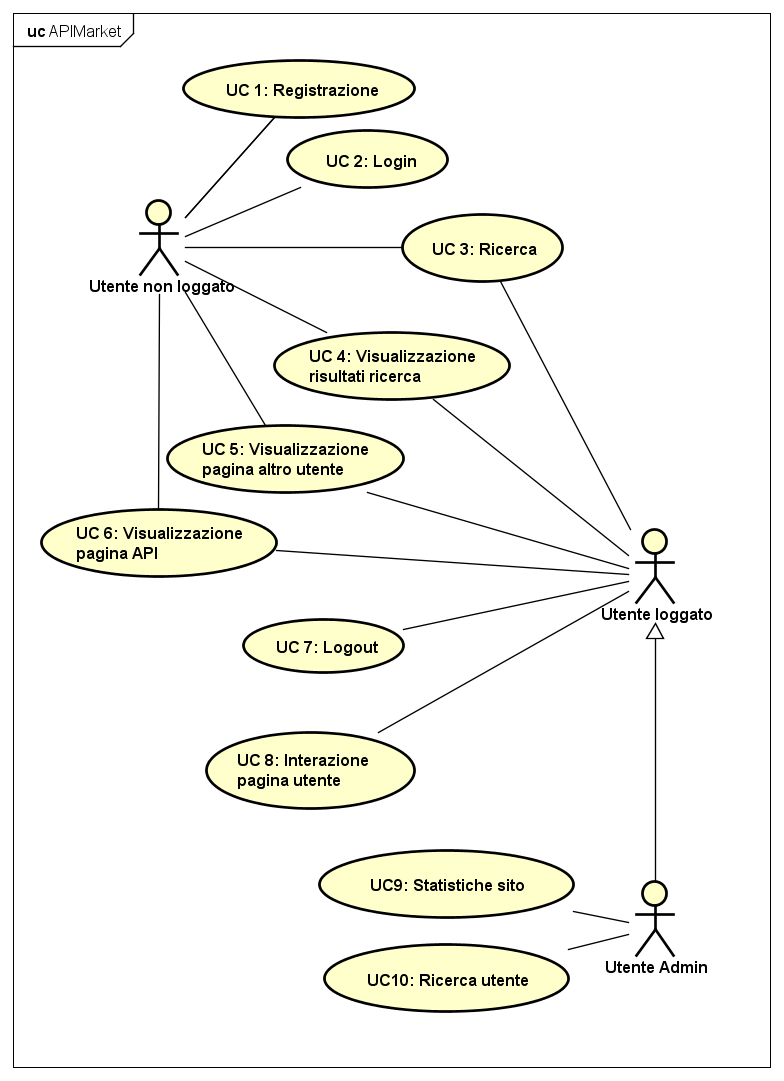
\includegraphics[width=0.7\textwidth]{UseCase/APIMarket}
	\caption{Operazioni ad alto livello}
\end{figure}
\begin{itemize}
	\item \textbf{Attori:} Utente non autenticato
	\item \textbf{Scopo e descrizione:} La pagina presenta tutti i servizi che sono offerti a un utente non autenticato ovvero:
	\begin{itemize} 
		\item Viene offerta la possibilità di registrarsi al market; 
		\item Viene offerta la possibilità di identificarsi se già in possesso di un account all'interno del market;
		\item Viene offerta la possibilità di consultare, solo a scopo informativo, le API all'interno del market (per poter caricare le proprie API, o acquistare APIKey è necessario accere con il proprio account); 
		\item Viene offerta la possibilità di consultare le statistiche riferite agli utenti all'interno del market;
	\end{itemize}
	\item \textbf{Precondizione:} Il sistema viene avviato da un utente esterno
	\item \textbf{Postcondizione:} Il sistema offre tutti servizi che un utente non autenticato può usufruire
\end{itemize}
\subsection{Caso d'uso UC1: Registrazione}
\begin{figure}[ht]
	\centering
	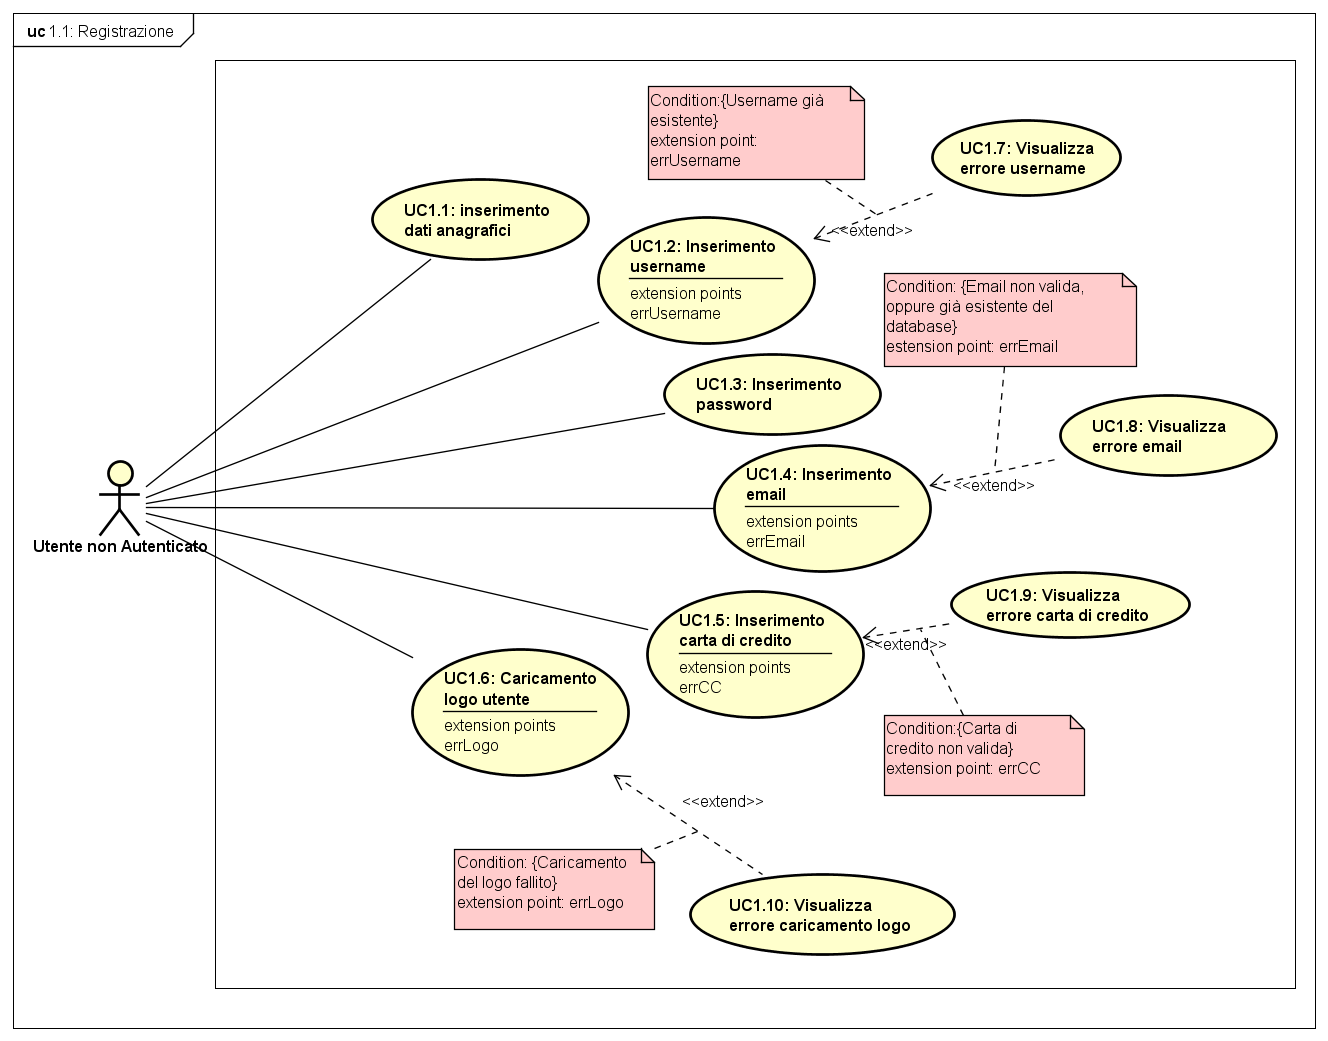
\includegraphics[width=0.7\textwidth]{UseCase/Registrazione}
	\caption{Registrazione}
\end{figure}
\begin{itemize}
	\item \textbf{Attori: Utente non autenticato}
	\item \textbf{Scopo e descrizione:} L'utente non i possesso di uno username e una password inserisce i suoi dati anagrafici da associare al nuovo username, gli verrà chiesta anche una password che dovrà utilizzare ogni qual volta debba effettare l'accesso;
	\item \textbf{Scenari alternativi:} Scenari alternativi: L'inserimento viene annullato per i seguenti motivi:
	\begin{itemize}
		\item username già esistente;
		\item password non soddisfa i criteri esposti. In tal caso viene richiesto all'utente di ripetere l'operazione.
	\end{itemize}
	\item \textbf{Precondizione:} Il sistema attende l'inserimento dei dati richiesti;
	\item \textbf{Postcondizione:} Il sistema si salva le informazione date dall'utente.
\end{itemize}
\subsection{Caso d'uso UC1.1: Inserimento dai anagrafici}
\begin{figure}[ht]
	\centering
	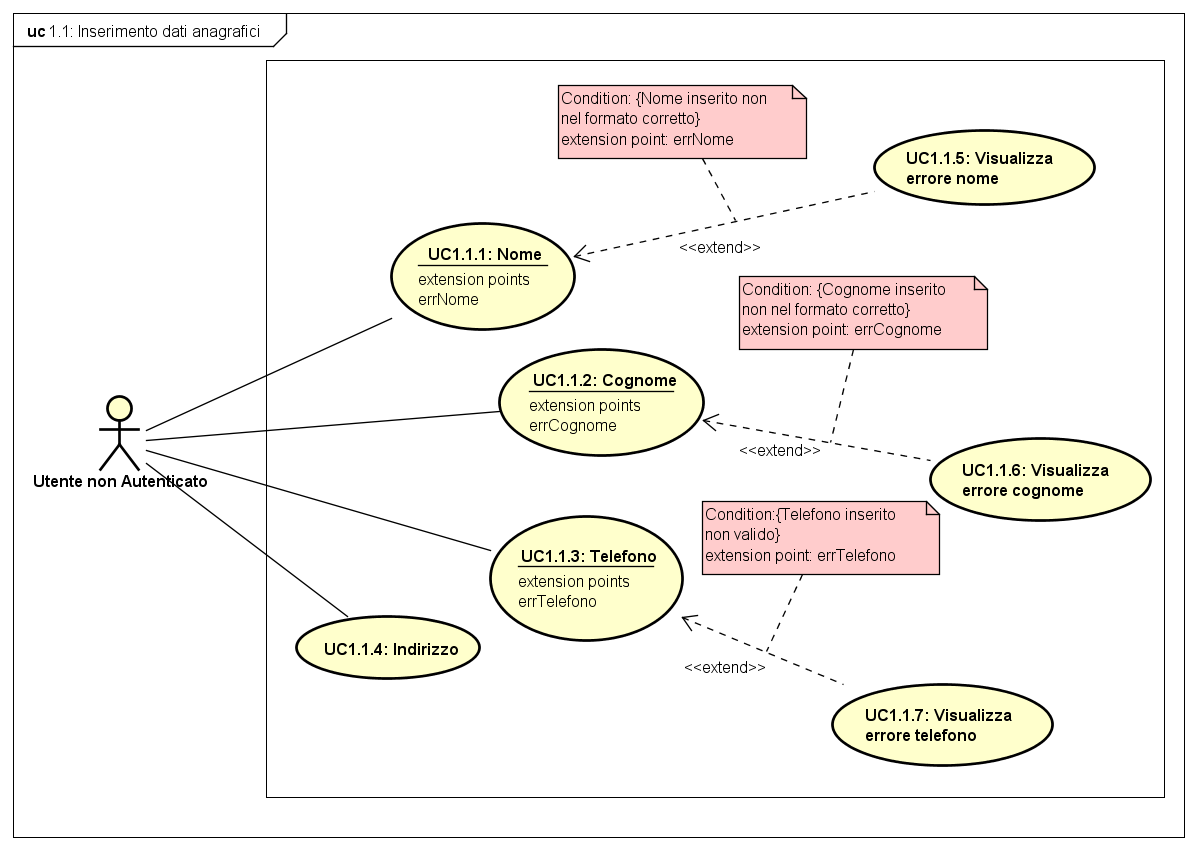
\includegraphics[width=0.7\textwidth]{UseCase/InserimentoDatiAnagrafici}
	\caption{Inserimento dati anagrafici}
\end{figure}
\begin{itemize}
	\item \textbf{Attori:} Utente non autenticato;
	\item \textbf{Scopo e descrizione:} L'utente non ancora autenticato inserisce i propri dati anagrafici (nome, cognome, nazionalità);
	\item \textbf{Precondizione:} Il sistema attende l'inserimento dei dati richiesti;
	\item \textbf{Postcondizione:} Il sistema salva le informazione date dall'utente.
\end{itemize}
\subsection{Caso d'uso UC1.1.1: Inserimento del nome}
\begin{itemize}
	\item \textbf{Attori:} Utente non autenticato; 
	\item \textbf{Scopo e descrizione:} L'utente deve inserire il suo nome;
	\item \textbf{Scenario alternativo:} Il nome inserito dall'utente non è conforme al formato richiesto;
	\item \textbf{Precondizione:} Il sistema attende l'inserimento del nome da parte dell'utente;
	\item \textbf{Postcondizione:} Il sistema inserisce nel DB il nome dell'utente.
\end{itemize}
\subsection{Caso d'uso UC1.1.2: Inserimento del cognome}
\begin{itemize}
	\item \textbf{Attori:} Utente non autenticato;
	\item \textbf{Scopo e descrizione:} L'utente deve inserire il suo nome;
	\item \textbf{Scenario alternativo:} Il nome inserito dall'utente non è conforme al formato richiesto;
	\item \textbf{Precondizione:} Il sistema attende l'inserimento del nome da parte dell'utente;
	\item \textbf{Postcondizione:} Il sistema inserisce nel DB il nome dell'utente.
\end{itemize}
\subsection{Caso d'uso UC1.1.3: Inserimento del telefono}
\begin{itemize}
	\item \textbf{Attori:} Utente non autenticato;
	\item \textbf{Scopo e descrizione:} L'utente deve inserire il suo numero di telefono;
	\item \textbf{Scenario alternativo:} Il numero di telefono inserito dall'utente non è valido;
	\item \textbf{Precondizione:} Il sistema attende l'inserimento del numero di telefono da parte dell'utente;
	\item \textbf{Postcondizione:} Il sistema inserisce nel DB il numero di telefono dell'utente.
\end{itemize}
\subsection{Caso d'uso UC1.1.4: Inserimento paese}
\begin{itemize}
	\item \textbf{Attori:} Utente non autenticato;
	\item \textbf{Scopo e descrizione:} L'utente deve inserire la nazionalità di appartenenza;
	\item \textbf{Scenario alternativo:} La nazionalità espressa dall'utente non esiste;
	\item \textbf{Precondizione:} Il sistema attende che l'utente scelga la nazionalità;
	\item \textbf{Postcondizione: }Il sistema inserisce nel DB il numero di telefono dell'utente.
\end{itemize}
\subsection{Caso d'uso UC1.2: Inserimento nome utente}
\begin{itemize}
	\item \textbf{Attori: }Utente non autenticato;
	\item \textbf{Scopo e descrizione: }L'utente inserisce lo username che gli servirà ad identificarsi nel sistema nel futuro;
	\item \textbf{Scenario alternativo: }Il sistema rifiuta lo username dato in quanto già presente nel DB, in tal caso viene chiesto di inserire all'utente un diverso username;
	\item \textbf{Precondizione: }Il sistema rimane in attesa dell'inserimento dello username;
	\item \textbf{Postcondizione: }Il sistema associa allo username i data anagrafici inseriti in precedenza e inserisce lo username nel DB degli utenti.
\end{itemize}
\subsection{Caso d'uso UC1.3: Inserimento password (Registrazione)}
\begin{figure}[H]
	\centering
	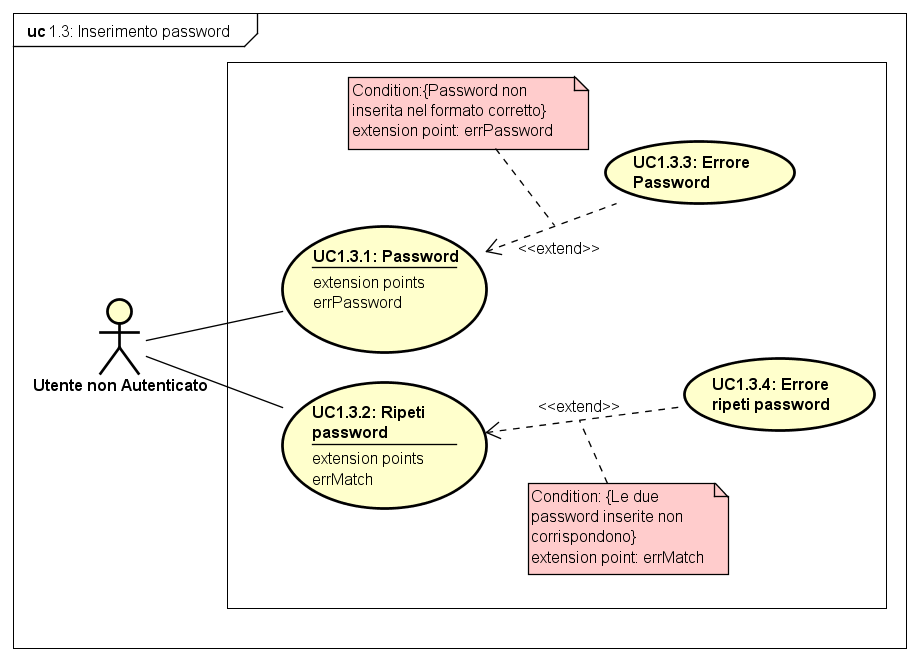
\includegraphics[width=0.7\textwidth]{UseCase/InserimentoPassword}
	\caption{Inserimento password (Registrazione)}
\end{figure}
\begin{itemize}
	\item \textbf{Attori: }Utente non autenticato;
	\item \textbf{Scopo e descrizione: } L'utente non autenticato inserisce una password che gli servirà come chiave di sicurezza per identificarsi nel sistema. La password richiesta, per poter essere accettata deve soddisfare i seguenti requisiti: 
	\begin{itemize}
		\item Deve essere lunga almeno 8 caratteri; 
		\item Deve contenere almeno 1 carattere maiuscolo; 
		\item Deve contere almeno 1 carattere minuscolo;
	\end{itemize}
	Inoltre la password inserita deve essere ripetuta come controllo di sicurezza.
	\item \textbf{Scenario alternativo: }La password inserita dall'utente non è conforme alle richieste, perciò il sistema chiede all'utente di inserire una nuova password che sia conforme, oppure la password ripetuta non combacia.
	\item \textbf{Precondizione: }Il sistema attende che l'utente inserisca la password da associare al suo username;
	\item \textbf{Postcondizione: }Il sistema accetta la password inserita dall'utente e la associa allo username nel DB corrispondente.
\end{itemize}
\subsection{Caso d'uso UC1.3.1: Password}
\begin{itemize}
	\item \textbf{Attori: }Utente non loggato;
	\item \textbf{Scopo e descrizione: }L'utente deve inserire la sua password con cui accederà al suo account una volta terminata la registrazione;
	\item \textbf{Scenario alternativo: }La password inserita non rispetta i requisiti minimi, viene quindi mostrato un messaggio d'errore;
	\item \textbf{Precondizione: }L'utente è nella schermata di registrazione e deve inserire la password;
	\item \textbf{Postcondizione: }L'utente ha inserito una password valida.
\end{itemize}
\subsection{Caso d'uso UC1.3.2: Ripeti password}
\begin{itemize}
	\item \textbf{Attori: }Utente non autenticato;
	\item \textbf{Scopo e descrizione: }L'utente deve reinserire la password come controllo di sicurezza;
	\item \textbf{Scenario alternativo: }L'utente ha inserito una password che non combacia con la password inserita in precedenza, viene quindi mostrato un messaggio di errore;
	\item \textbf{Precondizione: }L'utente è nella schermata di registrazione e ha inserito la password, deve inserire la password una seconda volta;
	\item \textbf{Postcondizione: }L'utente ha inserito la password per la seconda volta.
\end{itemize}
\subsection{Caso d'uso UC1.4: Inserimento email}
\begin{itemize}
	\item \textbf{Attori: }Utente non autenticato;
	\item \textbf{Scopo e descrizione: }Nel fututro nel caso in cui l'utente si fosse dimenticato la password, è necessario che il sistema abbia a disposizione un'email alla quale fare affidamento a cui poter mandare la password per poter far accedere l'utente;
	\item \textbf{Scenario alternativo: }L'email inserita non è nel formato valido, o esiste già nel database, quindi il sistema chiede all'utente di inserire un'altra email valida;
	\item \textbf{Precondizione: }Il sistema attende una email dall'utente;
	\item \textbf{Postcondizione: }Il sistema riceve una email che assocerà allo user name dell'utente.
\end{itemize}
\subsection{Caso d'uso UC1.5: Inserimento carta di credito}
\begin{itemize}
	\item \textbf{Attori: }Utente non autenticato;
	\item \textbf{Scopo e descrizione: }L'utente deve disporre di un metodo di una carta di credito valida che gli permetta di effettuare acquisti all'interno del market;
	\item \textbf{Scenario alternativo: }La carta di credito non è valida perciò viene segnalato errore e viene chiesto all'utente di inserirne uno diversa;
	\item \textbf{Precondizione: }Il sistema attende che l'utente inserisca una carta di credito valida;
	\item \textbf{Postcondizione: }Il sistema valida la carta di credito inserita dall'utente e la associa al suo account.
\end{itemize}
\subsection{Caso d'uso UC2: Login}
\begin{figure}[H]
	\centering
	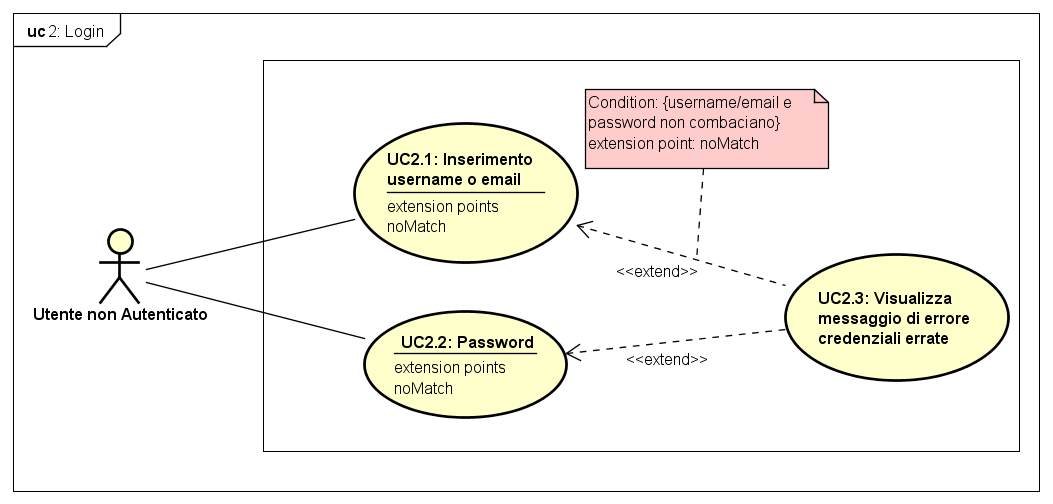
\includegraphics[width=0.7\textwidth]{UseCase/Login}
	\caption{Login}
\end{figure}
\begin{itemize}
	\item \textbf{Attori:} Utente non autenticato;
	\item \textbf{Scopo e descrizione:} L'utente che possiede già uno username e una password vuole effettuare un accesso;
	\item \textbf{Scenario alternativo: }Il sistema rifiuta l'accesso all'utente a causa di un errato inserimento di username o di password;
	\item \textbf{Precondizione: }Il sistema attende che l'utente inserisca i suoi dati identificativi;
	\item \textbf{Postcondizione: Il sistema ha accettato i dati e manda l'utente alla sua bacheca personale}.
\end{itemize}
\subsection{Caso d'uso UC2.1: Inserimento username o email}
\begin{itemize}
	\item \textbf{Attori: }Utente non autenticato;
	\item \textbf{Scopo e descrizione: }Viene chiesto all'utente di inserire il suo username o la sua email per poter essere identificato;
	\item \textbf{Scenario alternativo: }Lo username o l'email non esistono all'interno del DB;
	\item \textbf{Precondizione: }Il sistema attende l'inserimento dello username o dell'email da parte dell'utente;
	\item \textbf{Postcondizione: }Il sistema ha riconosciuto l'utente e attende l'inserimento della password per validare l'accesso.
\end{itemize}
\subsection{Caso d'uso UC2.2: Password}
\begin{itemize}
	\item \textbf{Attori: }Utente non autenticato;
	\item \textbf{Scopo e descrizione: }Viene chiesto all'utente di inserire la password associata allo username (o alla relativa email);
	\item \textbf{Scenario alternativo: }La password inserita dall'utente non corrisponde alla password associata allo username perciò viene rifiutato l'accesso;
	\item \textbf{Precondizione: }Il sistema attende l'inserimento della password da parte dell'utente;
	\item \textbf{Postcondizione: }Il sistema ha verificato che la password inserita dall'utente è corretta perciò logga l'utente.
\end{itemize}
\subsection{Caso d'uso UC2.3: Recupero password}
\begin{itemize}
	\item \textbf{Attori: }Utente non autenticato;
	\item \textbf{Scopo e descrizione: }Nel caso in cui l'utente si fosse dimenticato la password del suo profilo, il sistema offre un'assistenza di recupero password, ovvero invierà alla mail associata al profilo una nuova password temporanea da utilizzare per accedervi e modificarla nuovamente;
	\item \textbf{Precondizione: }Il sistema rimane in attesa della richiesta da parte dell'utente di recuperare la sua password;
	\item \textbf{Postcondizione: }L'utente ha a disposizione una password temporanea che gli permette di accedere al suo profilo e modificarla nuovamente.
\end{itemize}
\subsection{Caso d'uso UC3: Ricerca}
\begin{figure}[H]
	\centering
	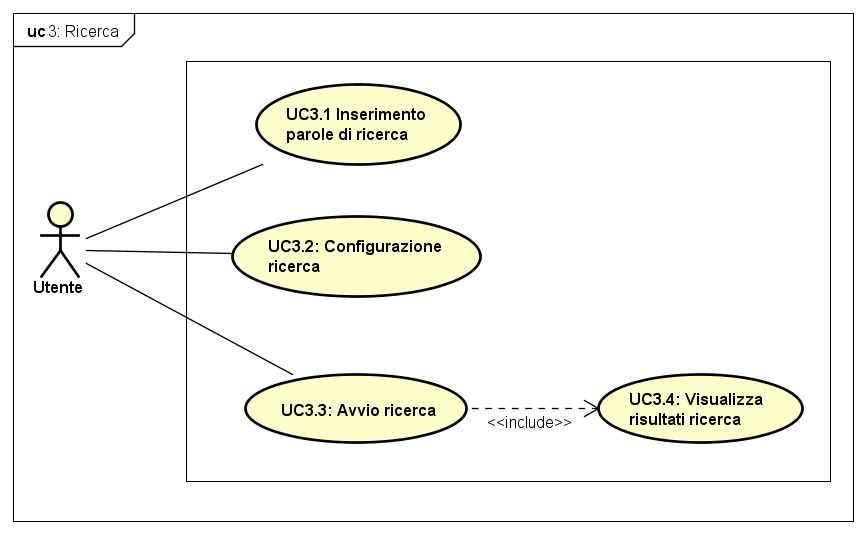
\includegraphics[width=0.7\textwidth]{UseCase/Ricerca}
	\caption{Ricerca}
\end{figure}
\begin{itemize}
	\item \textbf{Attori: }Utente non autenticato e Utente autenticato;
	\item \textbf{Scopo e descrizione: }L'utente ricerca nella barra di ricerca il nome di un microservizio e clicca il bottone di conferma;
	\item \textbf{Precondizione: }Il sistema attende l'invio di una frase di ricerca;
	\item \textbf{Postcondizione: }Il sistema ha esaminato la frase di ricerca e restituisce una pagina di risultati della ricerca.
\end{itemize}
\subsection{Caso d'uso UC3.1: Inserimento parole di ricerca}
\begin{itemize}
	\item \textbf{Attori: }Utente non autenticato e Utente autenticato;
	\item \textbf{Scopo e descrizione: }L'utente scrive nella barra di ricerca la frase che vuole ricercare;
	\item \textbf{Precondizione: }Il sistema attende l'inserimento di una frase di ricerca;
	\item \textbf{Postcondizione: }L'utente ha terminato di inserire la frase di ricerca.
\end{itemize}
\subsection{Caso d'uso UC3.2: Configurazione ricerca}
\begin{figure}[H]
	\centering
	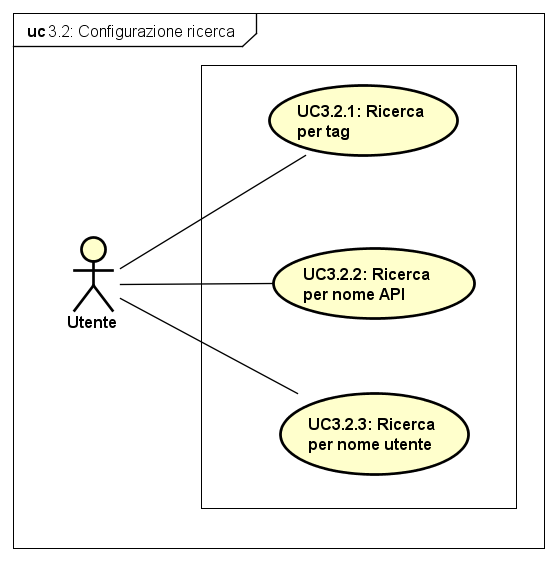
\includegraphics[width=0.7\textwidth]{UseCase/ConfigurazioneRicerca}
	\caption{Configurazione ricerca}
\end{figure}
\begin{itemize}
	\item \textbf{Attori: }Utente non autenticato e Utente autenticato;
	\item \textbf{Scopo e descrizione: }L'utente seleziona la modalità con cui vuole eseguire la ricerca;
	\item \textbf{Precondizione: }L'utente non ha ancora scelto nessun metodo di ricerca;
	\item \textbf{Postcondizione: }L'utente ha scelto un metodo di ricerca.
\end{itemize}
\subsection{Caso d'uso UC3.2.1: Ricerca per tag}
\begin{itemize}
	\item \textbf{Attori: }Utente non autenticato e Utente autenticato;
	\item \textbf{Scopo e descrizione: }L'utente sceglie di cercare all'interno di una categoria precisa di API;
	\item \textbf{Precondizione: }L'utente non ha ancora scelto la configurazione ricerca;
	\item \textbf{Postcondizione: }L'utente ha scelto il tag su cui effettuare la ricerca.
\end{itemize}
\subsection{Caso d'uso UC3.2.2: Ricerca per nome API}
\begin{itemize}
	\item \textbf{Attori: }Utente non autenticato e Utente autenticato;
	\item \textbf{Scopo e descrizione: }L'utente sceglie di cercare tra tutti i nomi dei microservizi del database;
	\item \textbf{Precondizione: }L'utente non ha ancora scelto la configurazione ricerca;
	\item \textbf{Postcondizione: }L'utente ha scelto la modalità di ricerca per nome API.
\end{itemize}
\subsection{Caso d'uso UC3.2.3: Ricerca per nome utente}
\begin{itemize}
	\item \textbf{Attori: }Utente non autenticato e Utente autenticato;
	\item \textbf{Scopo e descrizione: }L'utente sceglie di ricercare API tramite il nome utente dell'autore;
	\item \textbf{Precondizione: }L'utente non ha ancora scelto la configurazione ricerca;
	\item \textbf{Postcondizione: }L'utente ha scelto la modalità di ricerca per nome dell'autore.
\end{itemize}
\subsection{Caso d'uso UC3.3: Avvio ricerca}
\begin{itemize}
	\item \textbf{Attori: }Utente non autenticato e Utente autenticato;
	\item \textbf{Scopo e descrizione: }L'utente ha impostato la ricerca e preme il tasto per l'avvio della ricerca;
	\item \textbf{Precondizione: }L'utente ha finito di impostare la ricerca;
	\item \textbf{Postcondizione: }L'utente ha avviato la ricerca.
\end{itemize}
\subsection{Caso d'uso UC4: Visualizzazione risultati ricerca}
\begin{itemize}
	\item \textbf{Attori: }Utente non autenticato e Utente autenticato;
	\item \textbf{Scopo e descrizione: }L'utente ha avviato una ricerca e viene reindirizzato alla pagina di visione dei risultati di ricerca. Qui vengono elencate tutti i microservizi attinenti alla sua ricerca, o viene visualizzato un messaggio nel caso la ricerca non abbia prodotto risultati.
	\item \textbf{Precondizione: }L'utente ha avviato una ricerca;
	\item \textbf{Postcondizione: }L'utente ha accesso a tutti i microservizi attinenti alla ricerca.
\end{itemize}
\subsection{Caso d'uso UC5: Visualizzazione pagina altro utente}
\begin{figure}[H]
	\centering
	\includegraphics[width=0.7\textwidth]{UseCase/VisualizzazionePaginaAltroUtente}
	\caption{Visualizzazione pagina altro utente}
\end{figure}
\begin{itemize}
	\item \textbf{Attori: }Utente non autenticato e Utente Autenticato;
	\item \textbf{Scopo e descrizione: }L'utente è arrivato sulla pagina profilo di un altro utente e ne visiona i dati personali;
	\item \textbf{Precondizione: }L'utente vuole visionare i dati di un utente che ha caricato un microservizio;
	\item \textbf{Postcondizione: }L'utente è sulla pagina utente dell'utente che vuole visionare.
\end{itemize}
\subsection{Caso d'uso UC5.1: Visualizza nome utente}
\begin{itemize}
	\item \textbf{Attori: }Utente non autenticato e Utente autenticato;
	\item \textbf{Scopo e descrizione: }L'utente vuole visionare i dati di un utente;
	\item \textbf{Precondizione: }L'utente si trova nella pagina di un altro utente;
	\item \textbf{Postcondizione: }Il sistema ha stampato su schermo il nome di quell'utente e l'utente l'ha visionato.
\end{itemize}
\subsection{Caso d'uso UC5.2: Visualizza commenti scritti}
\begin{itemize}
	\item \textbf{Attori: }Utente non autenticato e Utente autenticato;
	\item \textbf{Scopo e descrizione: }L'utente vuole visionare gli ultimi commenti scritti da un altro utente;
	\item \textbf{Precondizione: }L'utente si trova sulla pagina di un altro utente;
	\item \textbf{Postcondizione: }Il sistema ha mostrato su schermo gli ultimi 30 messaggi scritti dall'utente.
\end{itemize}
\subsection{Caso d'uso UC 5.3: Visualizza microservizi pubblicati}
\begin{itemize}
	\item \textbf{Attori: }Utente non autenticato e Utente autenticato;
	\item \textbf{Scopo e descrizione: }L'utente vuole visionare i microservizi pubblicati da un dato utente, quindi va sulla sua pagina utente e li visiona;
	\item \textbf{Precondizione: }L'utente è sulla pagina di un altro utente;
	\item \textbf{Postcondizione: }Il sistema ha stampato su schermo una tabella che indica i microservizi rilasciati dall'utente, la data di rilascio, e approssimativamente il numero di download.
\end{itemize}
\subsection{Caso d'uso UC5.4: Visualizza indice di affidabilità}
\begin{itemize}
	\item \textbf{Attori: }Utente non autenticato e Utente autenticato;
	\item \textbf{Scopo e descrizione: }L'utente vuole verificare l'attendibilità di un altro utente prima di acquistare un suo microservizio, quindi va sulla sua pagina e legge il suo indice di affidabilità;
	\item \textbf{Precondizione: }L'utente è sulla pagina di un altro utente;
	\item \textbf{Postcondizione: }Il sistema calcola un indice di affidabilità per l'utente basato sulla qualità dei microservizi caricati e sulla loro valutazione da parte degli utenti, e lo stampa su schermo.
\end{itemize}
\subsection{Caso d'uso UC5.5: Modifica dati utente (admin)}
\begin{figure}[H]
	\centering
	\includegraphics[width=0.9\textwidth]{UseCase/ModificaDatiUtenteAdmin}
	\caption{Modifica dati utente (admin)}
\end{figure}
\begin{itemize}
	\item \textbf{Attori: }Utente Admin;
	\item \textbf{Scopo e descrizione: }L'utente Admin che visiona la pagina di un altro utente decide di cambiare alcuni dati relativi a quell'utente;
	\item \textbf{Precondizione: }L'utente Admin è sulla pagina di un altro utente;
	\item \textbf{Postcondizione: }L'utente Admin ha modificato tutto ciò che voleva modificare.
\end{itemize}
\subsection{Caso d'uso UC5.5.1: Modifica nome}
\begin{itemize}
	\item \textbf{Attori: }Utente Admin;
	\item \textbf{Scopo e descrizione: }L'utente Admin vuole modificare il nome in un profilo utente;
	\item \textbf{Precondizione: }L'utente Admin si trova nella pagina di un altro utente;
	\item \textbf{Postcondizione: }L'utente admin ha modificato il nome registrato da quell'utente.
\end{itemize}
\subsection{Caso d'uso UC 5.5.2: Modifica cognome}
\begin{itemize}
	\item \textbf{Attori: }Utente Admin;
	\item \textbf{Scopo e descrizione: }L'utente Admin vuole modificare il cognome in un profilo utente;
	\item \textbf{Precondizione: }L'utente Admin si trova nella pagina di un altro utente;
	\item \textbf{Postcondizione: }L'utente Admin ha modificato il cognome registrato da quell'utente.
\end{itemize}
\subsection{Caso d'uso UC5.5.3: Modifica paese}
\begin{itemize}
	\item \textbf{Attori: }Utente Admin;
	\item \textbf{Scopo e descrizione: }L'utente Admin vuole modificare il paese in un profilo utente;
	\item \textbf{Precondizione: }L'utente Admin si trova nella pagina di un altro utente;
	\item \textbf{Postcondizione: }L'utente Admin ha modificato il paese registrato da quell'utente.
\end{itemize}
\subsection{Caso d'uso UC5.5.4: Modifica password}
\begin{itemize}
	\item \textbf{Attori: }Utente Admin;
	\item \textbf{Scopo e descrizione: }L'utente Admin vuole modificare la password in un profilo utente;
	\item \textbf{Precondizione: }L'utente Admin si trova nella pagina di un altro utente;
	\item \textbf{Postcondizione: }L'utente Admin ha modificato la password registrata da quell'utente.
\end{itemize}
\subsection{Caso d'uso UC5.5.5: Modifica numero di telefono}
\begin{itemize}
	\item \textbf{Attori: }Utente Admin;
	\item \textbf{Scopo e descrizione: }L'utente Admin vuole modificare il numero di telefono in un profilo utente;
	\item \textbf{Precondizione: }L'utente Admin si trova nella pagina di un altro utente;
	\item \textbf{Postcondizione: }L'utente Admin ha modificato il numero di telefono registrato da quell'utente.
\end{itemize}
\subsection{Caso d'uso UC5.5.6: Modifica carta di credito}
\begin{itemize}
	\item \textbf{Attori: }Utente Admin;
	\item \textbf{Scopo e descrizione: }L'utente Admin vuole modificare la carta di credito in un profilo utente;
	\item \textbf{Precondizione: }L'utente Admin si trova nella pagina di un altro utente;
	\item \textbf{Postcondizione: }L'utente Admin ha modificato la carta di credito registrato da quell'utente.
\end{itemize}
\subsection{Caso d'uso UC5.5.7: Elimina commento}
\begin{itemize}
	\item \textbf{Attori: }Utente Admin;
	\item \textbf{Scopo e descrizione: }L'utente Admin vuole eliminare un commento in un profilo utente;
	\item \textbf{Precondizione: }L'utente Admin si trova nella pagina di un altro utente;
	\item \textbf{Postcondizione: }L'utente Admin ha eliminato il commento scritto da quell'utente.
\end{itemize}
\subsection{Caso d'uso UC5.5.8: Modifica microservizio}
\begin{itemize}
	\item \textbf{Attori: };
	\item \textbf{Scopo e descrizione: };
	\item \textbf{Precondizione: };
	\item \textbf{Postcondizione: }.
\end{itemize}
\subsection{Caso d'uso UC5.5.9: Elimina utente}
\begin{itemize}
	\item \textbf{Attori: }Utente Admin;
	\item \textbf{Scopo e descrizione: }L'utente Admin vuole eliminare un profilo utente;
	\item \textbf{Precondizione: }L'utente Admin si trova nella pagina di un altro utente;
	\item \textbf{Postcondizione: }L'utente Admin ha eliminato il profilo utente.
\end{itemize}
\subsection{Caso d'uso UC5.5.10: Modifica email}
\begin{itemize}
	\item \textbf{Attori: }Utente Admin;
	\item \textbf{Scopo e descrizione: }L'utente Admin vuole modificare l'indirizzo email in un profilo utente;
	\item \textbf{Scenari alternativi: }L'utente Admin ha inserito una mail in formato non valido, compare quindi un messaggio di errore che lo avvisa.
	\item \textbf{Precondizione: }L'utente Admin si trova nella pagina di un altro utente;
	\item \textbf{Postcondizione: }L'utente Admin ha modificato l'indirizzo email registrato da quell'utente.
\end{itemize}
\subsection{Caso d'uso UC6: Visualizzazione pagina API}
\begin{figure}[H]
	\centering
	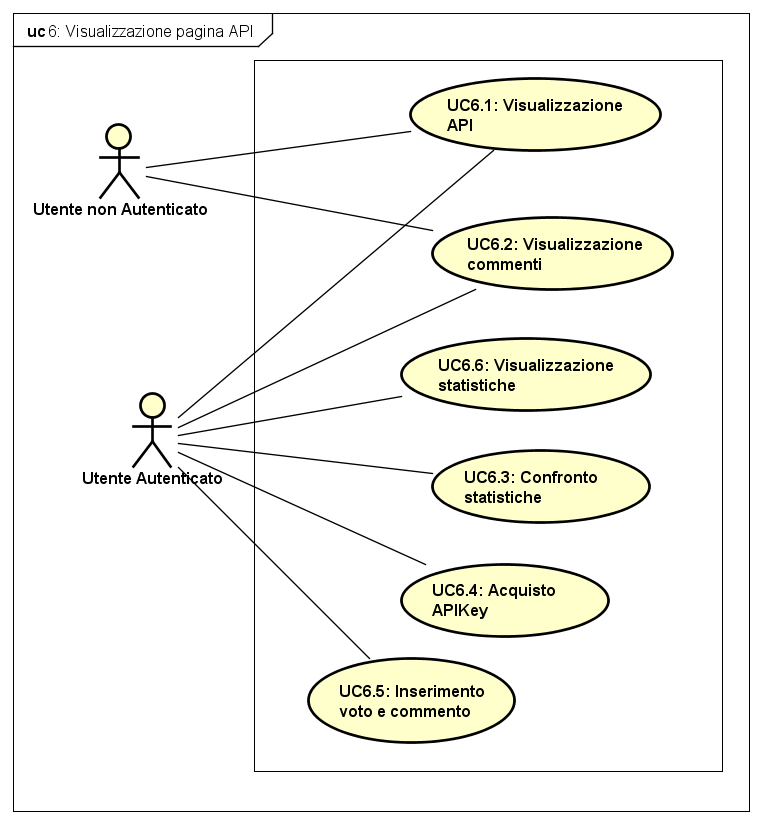
\includegraphics[width=0.8\textwidth]{UseCase/VisualizzazionePaginaAPI}
	\caption{Visualizzazione pagina API}
\end{figure}
\begin{itemize}
	\item \textbf{Attori: }Utente non autenticato e Utente autenticato;
	\item \textbf{Scopo e descrizione: }L'utente vuole visionare i dettagli di un microservizio registrato da un utente, apre quindi la pagina relativa a quel microservizio e la legge;
	\item \textbf{Precondizione: }L'utente ha cliccato sul nome di un microservizio;
	\item \textbf{Postcondizione: }L'utente è arrivato alla pagina di un microservizio e il sistema ha caricato tutte le informazioni relative.
\end{itemize}
\subsection{Caso d'uso UC 6.1: Visualizzazione API}
\begin{figure}[H]
	\centering
	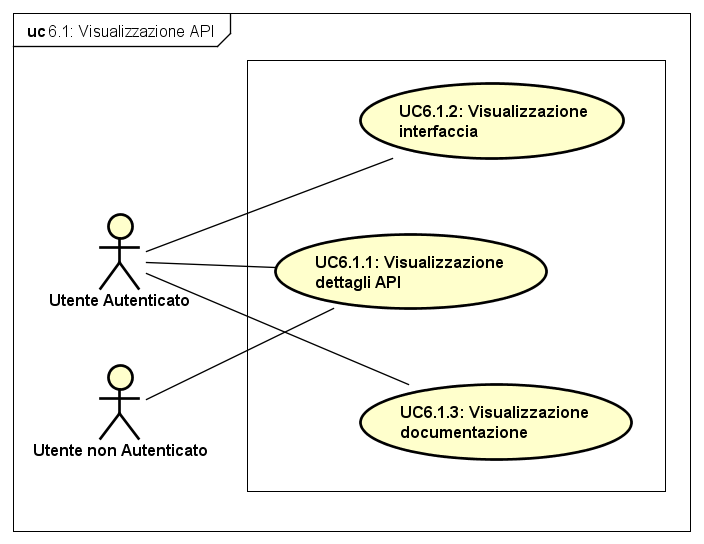
\includegraphics[width=0.7\textwidth]{UseCase/VisualizzazioneAPI}
	\caption{Visualizzazione API}
\end{figure}
\begin{itemize}
	\item \textbf{Attori: }Utente non autenticato e Utente autenticato;
	\item \textbf{Scopo e descrizione: }L'utente visualizza le informazioni principali relative al microservizio di cui gli interessano i dettagli;
	\item \textbf{Precondizione: }L'utente è sulla pagina di un microservizio;
	\item \textbf{Postcondizione: }Il sistema mostra all'utente le informazioni base su quel microservizio.
\end{itemize}
\subsection{Caso d'uso UC6.1.1: Visualizzazione nome}
\begin{itemize}
	\item \textbf{Attori: }Utente non autenticato e Utente Autenticato;
	\item \textbf{Scopo e descrizione: }L'utente legge il nome del microservizio di cui sta osservando la pagina;
	\item \textbf{Precondizione: }L'utente sta osservando la parte iniziale della pagina relativa ad un microservizio;
	\item \textbf{Postcondizione: }Il sistema ha caricato il nome di quel microservizio e lo ha stampato a schermo.
\end{itemize}
 \subsection{Caso d'uso UC6.1.2: Visualizzazione descrizione}
 \begin{itemize}
 	\item \textbf{Attori: }Utente non autenticato e Utente Autenticato;
 	\item \textbf{Scopo e descrizione: }L'utente legge la descrizione relativa al microservizio di cui sta osservando la pagina;
 	\item \textbf{Precondizione: }L'utente sta osservando la parte iniziale della pagina relativa ad un microservizio;
 	\item \textbf{Postcondizione: }Il sistema ha caricato il la descrizione relativa a quel microservizio e l'ha stampata a schermo.
 \end{itemize}
\subsection{Caso d'uso UC6.1.3: Visualizzazione rating}
\begin{itemize}
	\item \textbf{Attori: }Utente non autenticato e Utente Autenticato;
	\item \textbf{Scopo e descrizione: }L'utente legge la valutazione degli utenti relativa al microservizio di cui sta osservando la pagina;
	\item \textbf{Precondizione: }L'utente sta osservando la parte iniziale della pagina relativa ad un microservizio;
	\item \textbf{Postcondizione: }Il sistema ha caricato la valutazione degli utenti relativa a quel microservizio e l'ha stampata a schermo.
\end{itemize}
\subsection{Caso d'uso UC6.1.4: Visualizzazione intefaccia}
\begin{itemize}
	\item \textbf{Attori: }Utente autenticato;
	\item \textbf{Scopo e descrizione: }L'utente autenticato può visionare l'interfaccia di quel microservizio;
	\item \textbf{Precondizione: }L'utente sta osservando la parte iniziale della pagina relativa ad un microservizio;
	\item \textbf{Postcondizione: }Il sistema ha mostrato all'utente autenticato un link tramite il quale l'utente può osservare il file dell'interfaccia del microservizio.
\end{itemize}
\subsection{Caso d'uso UC6.1.5: Visualizzazione documentazione}
\begin{itemize}
	\item \textbf{Attori: }Utente autenticato;
	\item \textbf{Scopo e descrizione: }L'utente autenticato può osservare la documentazione relativa ad un microservizio;
	\item \textbf{Precondizione: }L'utente sta osservando la parte iniziale della pagina relativa ad un microservizio;
	\item \textbf{Postcondizione: }Il sistema ha mostrato all'utente autenticato un link tramite il quale l'utente può scaricare la documentazione del microservizio.
\end{itemize}
\subsection{Caso d'uso UC6.2: Visualizzazione commenti}
\begin{itemize}
	\item \textbf{Attori: }Utente non autenticato e Utente autenticato;
	\item \textbf{Scopo e descrizione: }L'utente che sta osservando la pagina di un microservizio può leggere i commenti degli altri utenti relativi a quel microservizio;
	\item \textbf{Precondizione: }L'utente è sulla pagina di un microservizio;
	\item \textbf{Postcondizione: }Il sistema mostra a schermo tutti i commenti relativi a quel microservizio, indicando anche il nome dell'autore del commento la data di pubblicazione.
\end{itemize}
\subsection{Caso d'uso UC6.3: Confronta statistiche}
\begin{itemize}
	\item \textbf{Attori: }Utente autenticato;
	\item \textbf{Scopo e descrizione: }L'utente autenticato vuole confrontare le statistiche del microservizio con quelle di un altro microservizio. Clicca sul bottone "confronta". Se ha già cliccato su un altro bottone "confronta" in precedenza allora viene reindirizzato ad una pagina in cui vedere il confronto, altrimenti il bottone rimane cliccato in attesa che l'utente prema il bottone "confronta" del microservizio che vuole mettere al confronto.
	\item \textbf{Precondizione: }L'utente sulla pagina di un microservizio clicca sul bottone "confronta";
	\item \textbf{Postcondizione: }Il sistema ha restituito all'utente le statistiche confrontate dei due microservizi scelti dall'utente, oppure ha mantenuto cliccato il pulsante avvisando l'utente di cliccare sul pulsante "confronta" relativo al microservizio che vuole mettere a confronto.
\end{itemize}
\subsection{Caso d'uso UC6.4: Acquisto APIKey}
\begin{itemize}
	\begin{figure}[H]
		\centering
		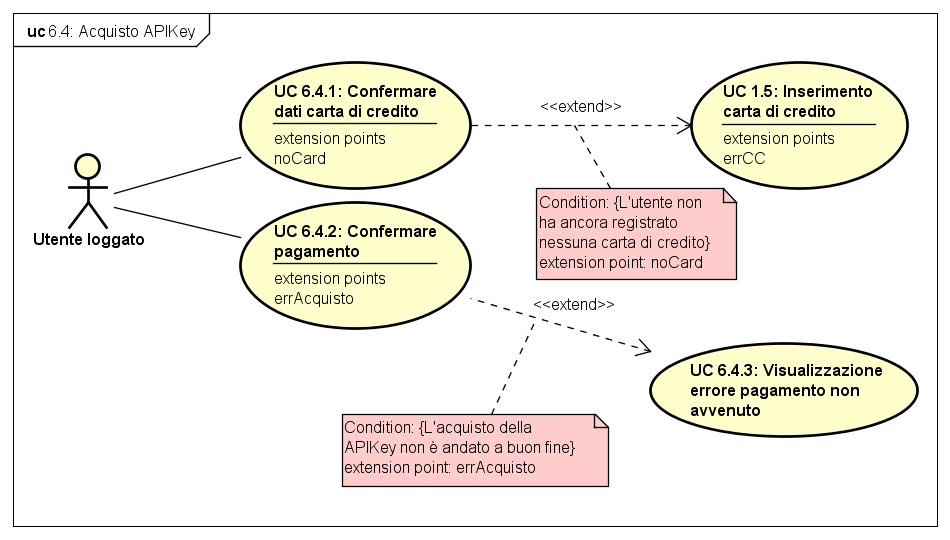
\includegraphics[width=0.8\textwidth]{UseCase/AcquistoAPIKey}
		\caption{Acquisto APIKey}
	\end{figure}
	\item \textbf{Attori: }Utente autenticato;
	\item \textbf{Scopo e descrizione: }L'utente autenticato vuole acquistare una APIKey, quindi preme sul pulsante di acquisto. Viene reindirizzato nella pagina di conferma di acquisto nel caso abbia una carta di credito registrata nel suo account, altrimenti viene reindirizzato nella pagina per registrare una carta di credito.
	\item \textbf{Scenari alternativi: }L'utente non ha registrato nessuna carta di credito sul suo account, viene quindi reindirizzato alla pagina di registrazione di una carta di credito.
	\item \textbf{Precondizione: }L'utente autenticato ha cliccato sul pulsante per acquistare una APIKey nella pagina di un microservizio;
	\item \textbf{Postcondizione: }L'utente viene condotto nella pagina di conferma di acquisto.
\end{itemize}
\subsection{Caso d'uso UC6.4.1: Confermare carta di credito}
\begin{itemize}
	\item \textbf{Attori: }Utente autenticato;
	\item \textbf{Scopo e descrizione: }L'utente decide se confermare la sua carta di credito registrata nel suo account o se cambiarla;
	\item \textbf{Scenario alternativo: }L'utente decide di cambiare la carta di credito con cui effettuare l'acquisto, viene quindi reindirizzato ad una pagina in cui inserire una carta di credito.
	\item \textbf{Precondizione: }L'utente è nella pagina di conferma di acquisto;
	\item \textbf{Postcondizione: }L'utente ha una carta di credito valida con cui effettuare il pagamento.
\end{itemize}
\subsection{Caso d'uso UC6.4.2: Confermare pagamento}
\begin{itemize}
	\item \textbf{Attori: }Utente autenticato;
	\item \textbf{Scopo e descrizione: }L'utente conferma il pagamento cliccando sul pulsante di conferma, viene reindirizzato su una pagina che annuncia l'esito dell'operazione e, se l'operazione è andata a buon fine, visualizza la sua nuova APIkey;
	\item \textbf{Scenario alternativo: }L'operazione non va a buon fine, viene quindi visualizzato un messaggio di errore transazione non eseguita;
	\item \textbf{Precondizione: }L'utente ha cliccato sul pulsante di conferma pagamento;
	\item \textbf{Postcondizione: }L'utente viene reindirizzato ad una pagina che descrive l'esito dell'operazione e, nel caso l'operazione sia andata a buon fine, visualizzi la sua APIkey.
\end{itemize}
\subsection{Caso d'uso UC6.5: Inserimento voto e commento}
\begin{itemize}
	\item \textbf{Attori: }Utente autenticato;
	\item \textbf{Scopo e descrizione: }L'utente autenticato che ha acquistato una APIKey relativa al microservizio può rilasciare un commento e una valutazione che va da 1 a 5, e una volta scritto clicca sul pulsante di conferma;
	\item \textbf{Precondizione: }L'utente è sulla pagina di un microservizio;
	\item \textbf{Postcondizione: }Il sistema ricarica la pagina e aggiunge il nuovo commento.
\end{itemize}
\subsection{Caso d'uso UC6.6: Visualizzazione statistiche }
\begin{figure}[H]
	\centering
	\includegraphics[width=0.7\textwidth]{UseCase/VisualizzazioneStatistiche}
	\caption{Visualizzazione statistiche}
\end{figure}
\begin{itemize}
	\item \textbf{Attori: }Utente autenticato;
	\item \textbf{Scopo e descrizione: }L'utente vuole visualizzare le statistiche prestazionali di un microservizio, quindi clicca sul link apposito. Viene quindi visualizzata una pagina con tutte le statistiche cercate;
	\item \textbf{Precondizione: }L'utente è sulla pagina di un microservizio e clicca sul link di visione delle statistiche;
	\item \textbf{Postcondizione: }L'utente è stato reindirizzato alla pagina di visione delle statistiche del microservizio.
\end{itemize}
\subsection{Caso d'uso UC6.6.1: Numero APIKey vendute}
\begin{itemize}
	\item \textbf{Attori: }Utente autenticato;
	\item \textbf{Scopo e descrizione: }L'utente visualizza le statistiche del microservizio;
	\item \textbf{Precondizione: }L'utente è sulla pagina delle statistiche del microservizio;
	\item \textbf{Postcondizione: }Il sistema stampa a schermo il numero approssimativo delle APIKey vendute.
\end{itemize}
\subsection{Caso d'uso UC6.6.2: Tempo medio di risposta}
\begin{itemize}
	\item \textbf{Attori: }Utente autenticato;
	\item \textbf{Scopo e descrizione: }L'utente visualizza le statistiche del microservizio;
	\item \textbf{Precondizione: }L'utente è sulla pagina delle statistiche del microservizio;
	\item \textbf{Postcondizione: }Il sistema stampa a schermo il tempo medio di risposta del microservizio al netto dei ritardi introdotti dall'API Gateway.
\end{itemize}
\subsection{Caso d'uso UC6.6.3: Dati medi scambiati}
\begin{itemize}
	\item \textbf{Attori: }Utente autenticato;
	\item \textbf{Scopo e descrizione: }L'utente visualizza le statistiche del microservizio;
	\item \textbf{Precondizione: }L'utente è sulla pagina delle statistiche del microservizio;
	\item \textbf{Postcondizione: }Il sistema stampa a schermo il numero di dati medi scambiati mensili dal microservizio attraverso l'API Gateway.
\end{itemize}
\subsection{Caso d'uso UC6.6.4: Numero medio di chiamate}
\begin{itemize}
	\item \textbf{Attori: }Utente autenticato;
	\item \textbf{Scopo e descrizione: }L'utente visualizza le statistiche del microservizio;
	\item \textbf{Precondizione: }L'utente è sulla pagina delle statistiche del microservizio;
	\item \textbf{Postcondizione: }Il sistema stampa a schermo il numero medio di chiamate mensili al microservizio attraverso l'API Gateway.
\end{itemize}
\subsection{Caso d'uso UC7: Logout}
\begin{itemize}
	\item \textbf{Attori: }Utente autenticato;
	\item \textbf{Scopo e descrizione: }L'utente ha la possibilità di disconnetere il suo profilo dal sistema;
	\item \textbf{Precondizione: }L'utente ha acceduto alla sessione del sistema;
	\item \textbf{Postcondizione: }Il sistema ha disconnesso l'utente dalla sessione a cui apparteneva.
\end{itemize}
\subsection{Caso d'uso UC8: Interazione pagina utente}
\begin{figure}[H]
	\centering
	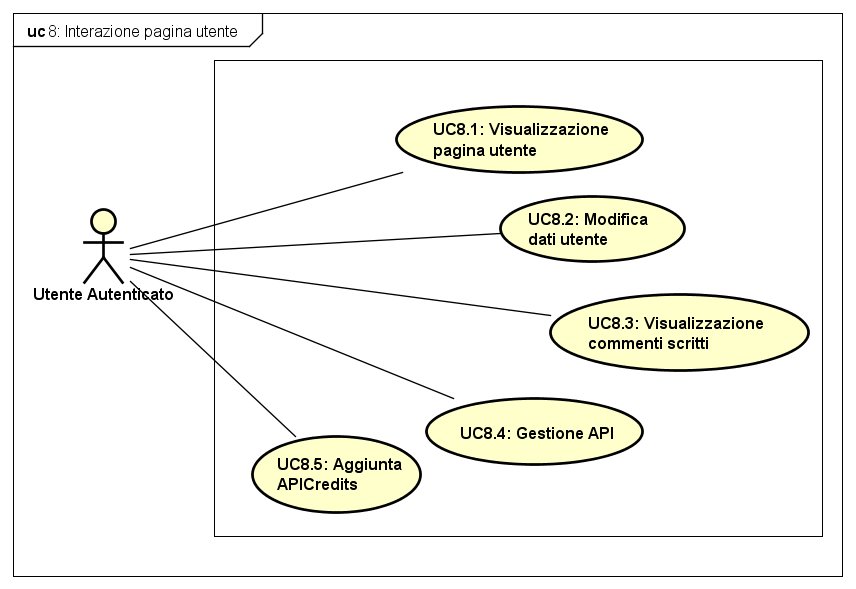
\includegraphics[width=0.7\textwidth]{UseCase/InterazionePaginaUtente}
	\caption{Interazione pagina utente}
\end{figure}
\begin{itemize}
	\item \textbf{Attori: }Utente autenticato;
	\item \textbf{Scopo e descrizione: }Un utente autenticato può visitare la sua pagina profilo per visualizzare i suoi dati, modificarli, visionare i suoi commenti scritti, registrare nuovi microservizi e vedere le loro statistiche;
	\item \textbf{Precondizione: }L'utente clicca sul suo profilo;
	\item \textbf{Postcondizione: }Il sistema apre la sua pagina utente.
\end{itemize}
\subsection{Caso d'uso UC 8.1: Visualizzazione pagina utente}
\begin{itemize}
	\item \textbf{Attori: }Utente autenticato;
	\item \textbf{Scopo e descrizione: }L'utente sulla sua pagina profilo può visionare tutti i suoi dati inseriti al momento della registrazione. In particolare può visualizzare:
	\begin{itemize}
		\item Nome utente;
		\item Nome e cognome;
		\item Indirizzo email;
		\item Numero di telefono;
		\item Paese di provenienza;
		\item Indice di affidabilità
	\end{itemize}
	\item \textbf{Precondizione: }L'utente è sulla sua pagina profilo;
	\item \textbf{Postcondizione: }Il sistema stampa su schermo tutte le informazioni personali dell'utente.
\end{itemize}
\subsection{Caso d'uso UC8.2: Modifica dati utente}
\begin{figure}[H]
	\centering
	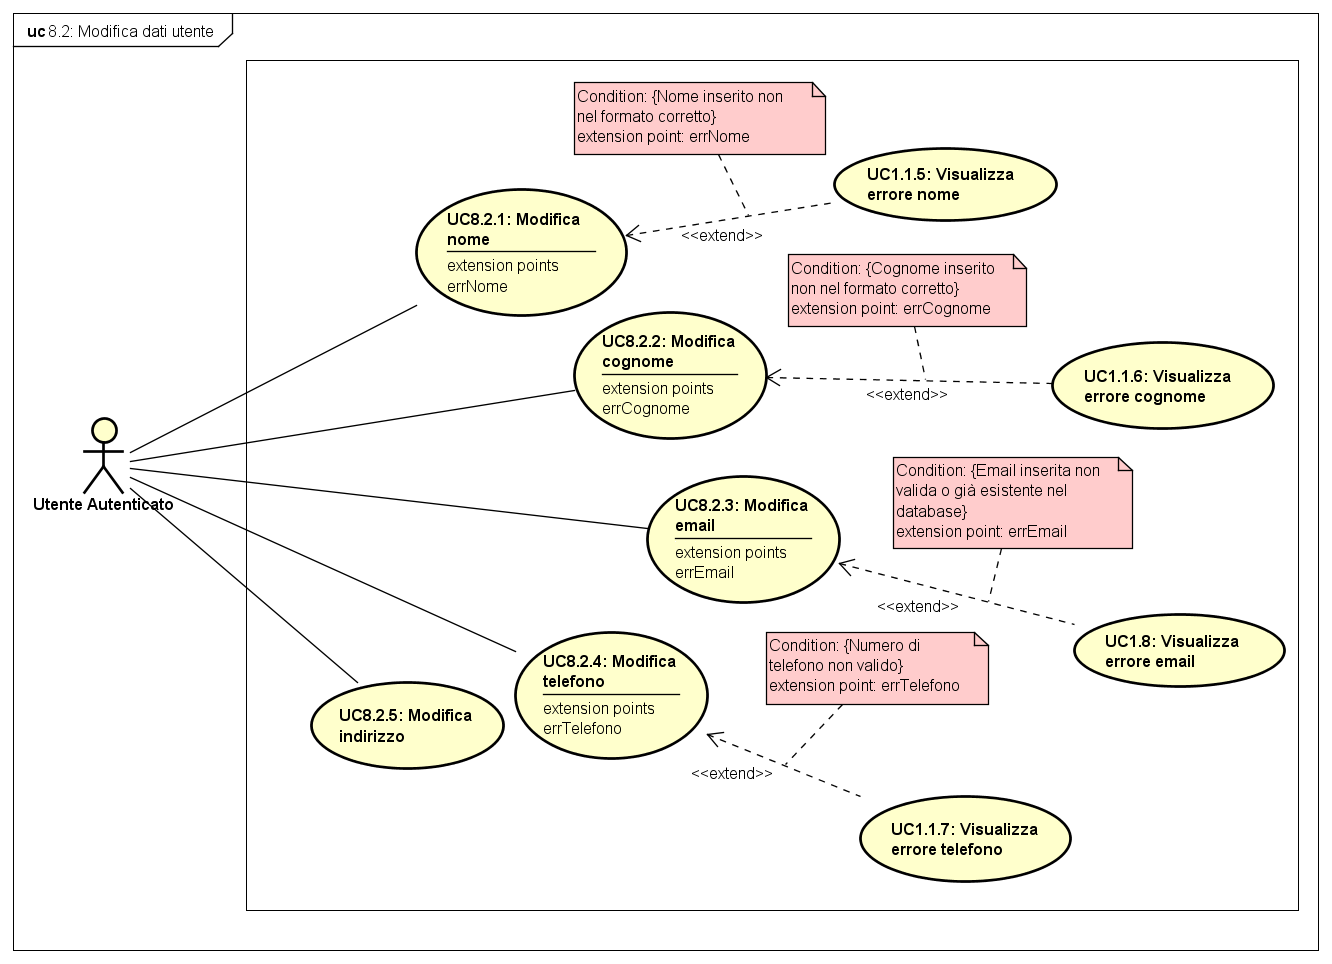
\includegraphics[width=0.8\textwidth]{UseCase/ModificaDatiUtente}
	\caption{Modifica dati utente}
\end{figure}
\begin{itemize}
	\item \textbf{Attori: }Utente autenticato;
	\item \textbf{Scopo e descrizione: }L'utente autenticato può modificare tutti i suoi dati ad eccezione del nome untente;
	\item \textbf{Precondizione: }L'utente è sulla sua pagina di profilo e clicca sul pulsante per la modifica dei suoi dati;
	\item \textbf{Postcondizione: }Il sistema ha permesso la modifica dei suoi dati.
\end{itemize}
\subsection{Caso d'uso UC8.2.1: Modifica nome}
\begin{itemize}
	\item \textbf{Attori: }Utente autenticato;
	\item \textbf{Scopo e descrizione: }L'utente autenticato può modificare il suo nome;
	\item \textbf{Scenario alternativo: }Il nome inserito non è nel formato corretto, il sistema quindi fornisce un errore all'utente;
	\item \textbf{Precondizione: }L'utente è sulla sua pagina utente ed ha cliccato il pulsante per la modifica dei suoi dati;
	\item \textbf{Postcondizione: }L'utente ha modificato i suoi dati.
\end{itemize}
\subsection{Caso d'uso UC8.2.2: Modifica cognome}
\begin{itemize}
	\item \textbf{Attori: }Utente autenticato;
	\item \textbf{Scopo e descrizione: }L'utente autenticato può modificare il suo cognome;
	\item \textbf{Scenario alternativo: }Il cognome inserito non è nel formato corretto, il sistema quindi fornisce un errore all'utente;
	\item \textbf{Precondizione: }L'utente è sulla sua pagina utente ed ha cliccato il pulsante per la modifica dei suoi dati;
	\item \textbf{Postcondizione: }L'utente ha modificato i suoi dati.
\end{itemize}
\subsection{Caso d'uso UC8.2.3: Modifica email}
\begin{itemize}
	\item \textbf{Attori: }Utente autenticato;
	\item \textbf{Scopo e descrizione: }L'utente autenticato può modificare il suo indirizzo email;
	\item \textbf{Scenario alternativo: }L'indirizzo email inserito non è nel formato corretto o esiste già nel database, il sistema quindi fornisce un errore all'utente;
	\item \textbf{Precondizione: }L'utente è sulla sua pagina utente ed ha cliccato il pulsante per la modifica dei suoi dati;
	\item \textbf{Postcondizione: }L'utente ha modificato i suoi dati.
\end{itemize}
\subsection{Caso d'uso UC8.2.4: Modifica telefono}
\begin{itemize}
	\item \textbf{Attori: }Utente autenticato;
	\item \textbf{Scopo e descrizione: }L'utente autenticato può modificare il suo numero di telefono;
	\item \textbf{Scenario alternativo: }Il numero di telefono inserito non è nel formato corretto, il sistema quindi fornisce un errore all'utente;
	\item \textbf{Precondizione: }L'utente è sulla sua pagina utente ed ha cliccato il pulsante per la modifica dei suoi dati;
	\item \textbf{Postcondizione: }L'utente ha modificato i suoi dati.
\end{itemize}
\subsection{Caso d'uso UC8.2.5: Modifica paese}
\begin{itemize}
	\item \textbf{Attori: }Utente autenticato;
	\item \textbf{Scopo e descrizione: }L'utente autenticato può modificare il suo paese;
	\item \textbf{Scenario alternativo: }Il paese inserito non è nel formato corretto, il sistema quindi fornisce un errore all'utente;
	\item \textbf{Precondizione: }L'utente è sulla sua pagina utente ed ha cliccato il pulsante per la modifica dei suoi dati;
	\item \textbf{Postcondizione: }L'utente ha modificato i suoi dati.
\end{itemize}
\subsection{Caso d'uso UC8.3: Visualizza commenti scritti}
\begin{itemize}
	\item \textbf{Attori: }Utente autenticato;
	\item \textbf{Scopo e descrizione: }L'utente autenticato visionando il suo profilo può leggere i commenti che ha scritto;
	\item \textbf{Precondizione: }L'utente è sulla sua pagina profilo;
	\item \textbf{Postcondizione: }Il sistema ha stampato su schermo tutti i commenti scritti dall'utente.
\end{itemize}
\subsection{Caso d'uso: UC8.4 Gestione API}
\begin{figure}[H]
	\centering
	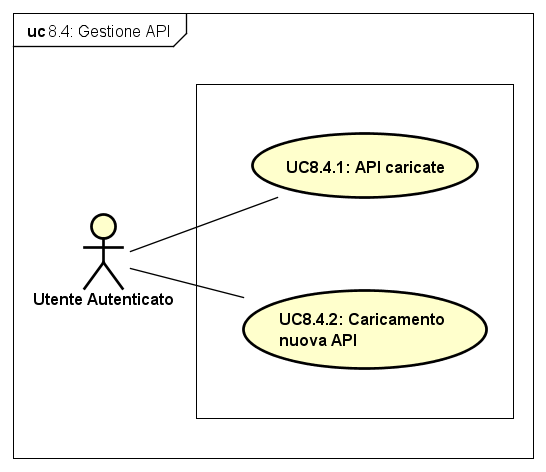
\includegraphics[width=0.5\textwidth]{UseCase/GestioneAPI}
	\caption{Gestione API}
\end{figure}
\begin{itemize}
	\item \textbf{Attori: }Utente autenticato;
	\item \textbf{Scopo e descrizione: }L'utente autenticato che visiona il suo profilo ha accesso ad una pagina in cui sono elencate tutti i microservizi da lui registrati, e per ciascuno di essi statistiche che descrivano le sue attività. Può inoltre registrare nuovi microservizi;
	\item \textbf{Precondizione: }L'utente è sulla sua pagina profilo;
	\item \textbf{Postcondizione: }Il sistema ha mostrato all'utente tutte le informazioni sui microservizi da lui caricati, e gli ha permesso di registrare i microservizi che voleva registrare.
\end{itemize}
\subsection{Caso d'uso UC8.4.1: Visualizza API caricate}
\begin{figure}[H]
	\centering
	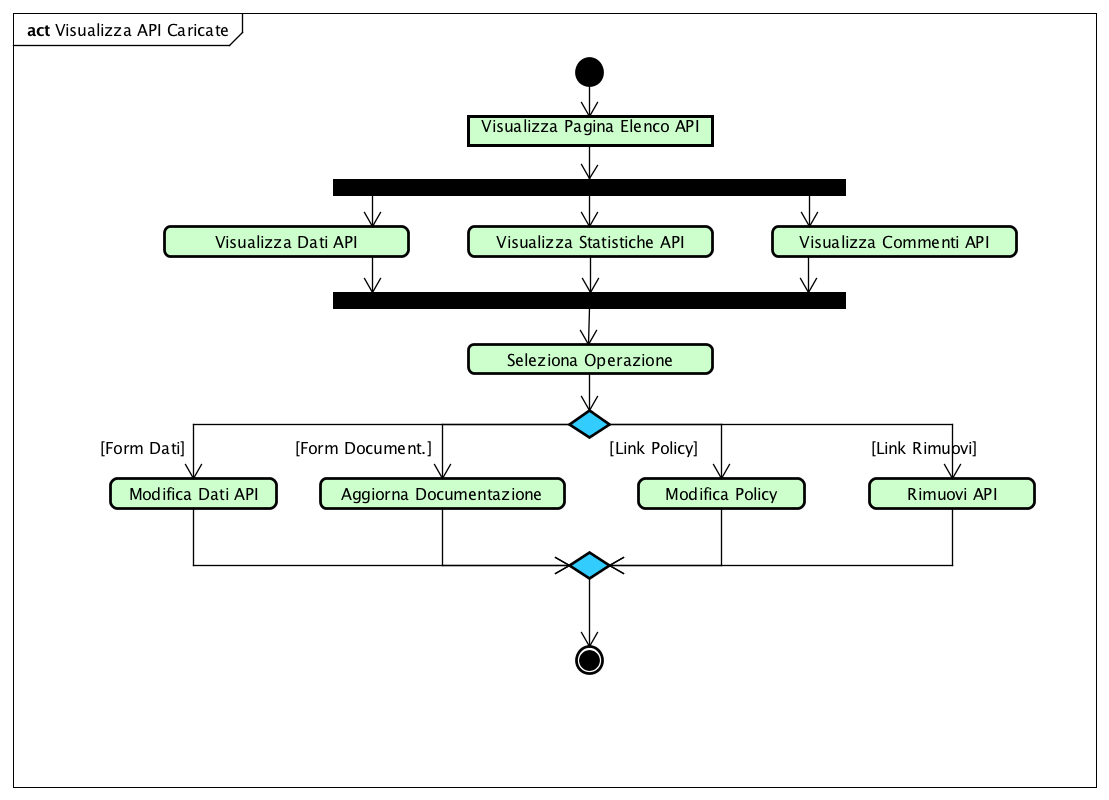
\includegraphics[width=0.7\textwidth]{UseCase/VisualizzaAPICaricate}
	\caption{Visualizza API caricate}
\end{figure}
\begin{itemize}
	\item \textbf{Attori: }Utente autenticato;
	\item \textbf{Scopo e descrizione: }L'utente autenticato nella sua pagina utente può visionare tutti i microservizi;
	\item \textbf{Precondizione: }L'utente è sulla sua pagina profilo;
	\item \textbf{Postcondizione: }Il sistema ha mostrato all'utente tutti i microservizi da lui registrati.
\end{itemize}
\subsection{Caso d'uso UC8.4.1.1: Visualizza Statistiche API}
\begin{itemize}
	\item \textbf{Attori: }Utente autenticato;
	\item \textbf{Scopo e descrizione: }L'utente può visionare tutte le statistiche relative ad un particolare microservizio che ha registrato. In particolare:
	\begin{itemize}
		\item Numero di APIKey vendute;
		\item Il guadagno totalo prodotto dal microservizio;
		\item Il guadagno medio mensile prodotto dal microservizio;
		\item L'elenco degli utenti in possesso di una APIKey relativa al microservizio;
		\item Il traffico totale prodotto dal microservizio attraverso l'API Gateway;
		\item Il traffico medio mensile prodotto dal microservizio attraverso l'API Gateway;
		\item L'indice di valutazione degli utenti relativo al microservizio;
		\item L'elenco di tutti commenti degli utenti relativi al microservizio;
		\item L'elenco dei crash commessi dal suo microservizio e notificati dall'API Gateway;
		\item Il tempo medio di risposta al netto del tempo di risposta dell'API Gateway;
		\item Il numero di chiamate totali al microservizio tramite APIKeys;
		\item il numero di chiamate medio mensile al microservizio tramite APIKeys.
	\end{itemize}
	\item \textbf{Precondizione: }L'utente è sulla sua pagina utente ed ha visionato tutti i suoi microservizi registrati;
	\item \textbf{Postcondizione: }Il sistema ha fornito all'utente tutte le statistiche relative al microservizio che interessa all'utente.
\end{itemize}
\subsection{Caso d'uso UC8.4.1.2: Modifica API}
\begin{itemize}
	\item \textbf{Attori: }Utente autenticato;
	\item \textbf{Scopo e descrizione: }L'utente può modificare le informazioni di un microservizio da lui registrato. In particolare può:
	\begin{itemize}
		\item Modificare la descrizione;
		\item Modificare l'interfaccia caricata;
		\item Modificare il logo del microservizio;
		\item Modificare il prezzo delle APIKey;
		\item Modificare la documentazione relativa.
	\end{itemize}
	\item \textbf{Precondizione: }L'utente sta visionando un microservizio che ha registrato e clicca sul pulsante di modifica dati;
	\item \textbf{Postcondizione: }Il sistema ha permesso all'utente di compiere le modifiche richieste.
\end{itemize}
\end{document}